\begin{landscape}\section{Elektrisch}

\begin{figure}[h]
	\centering
		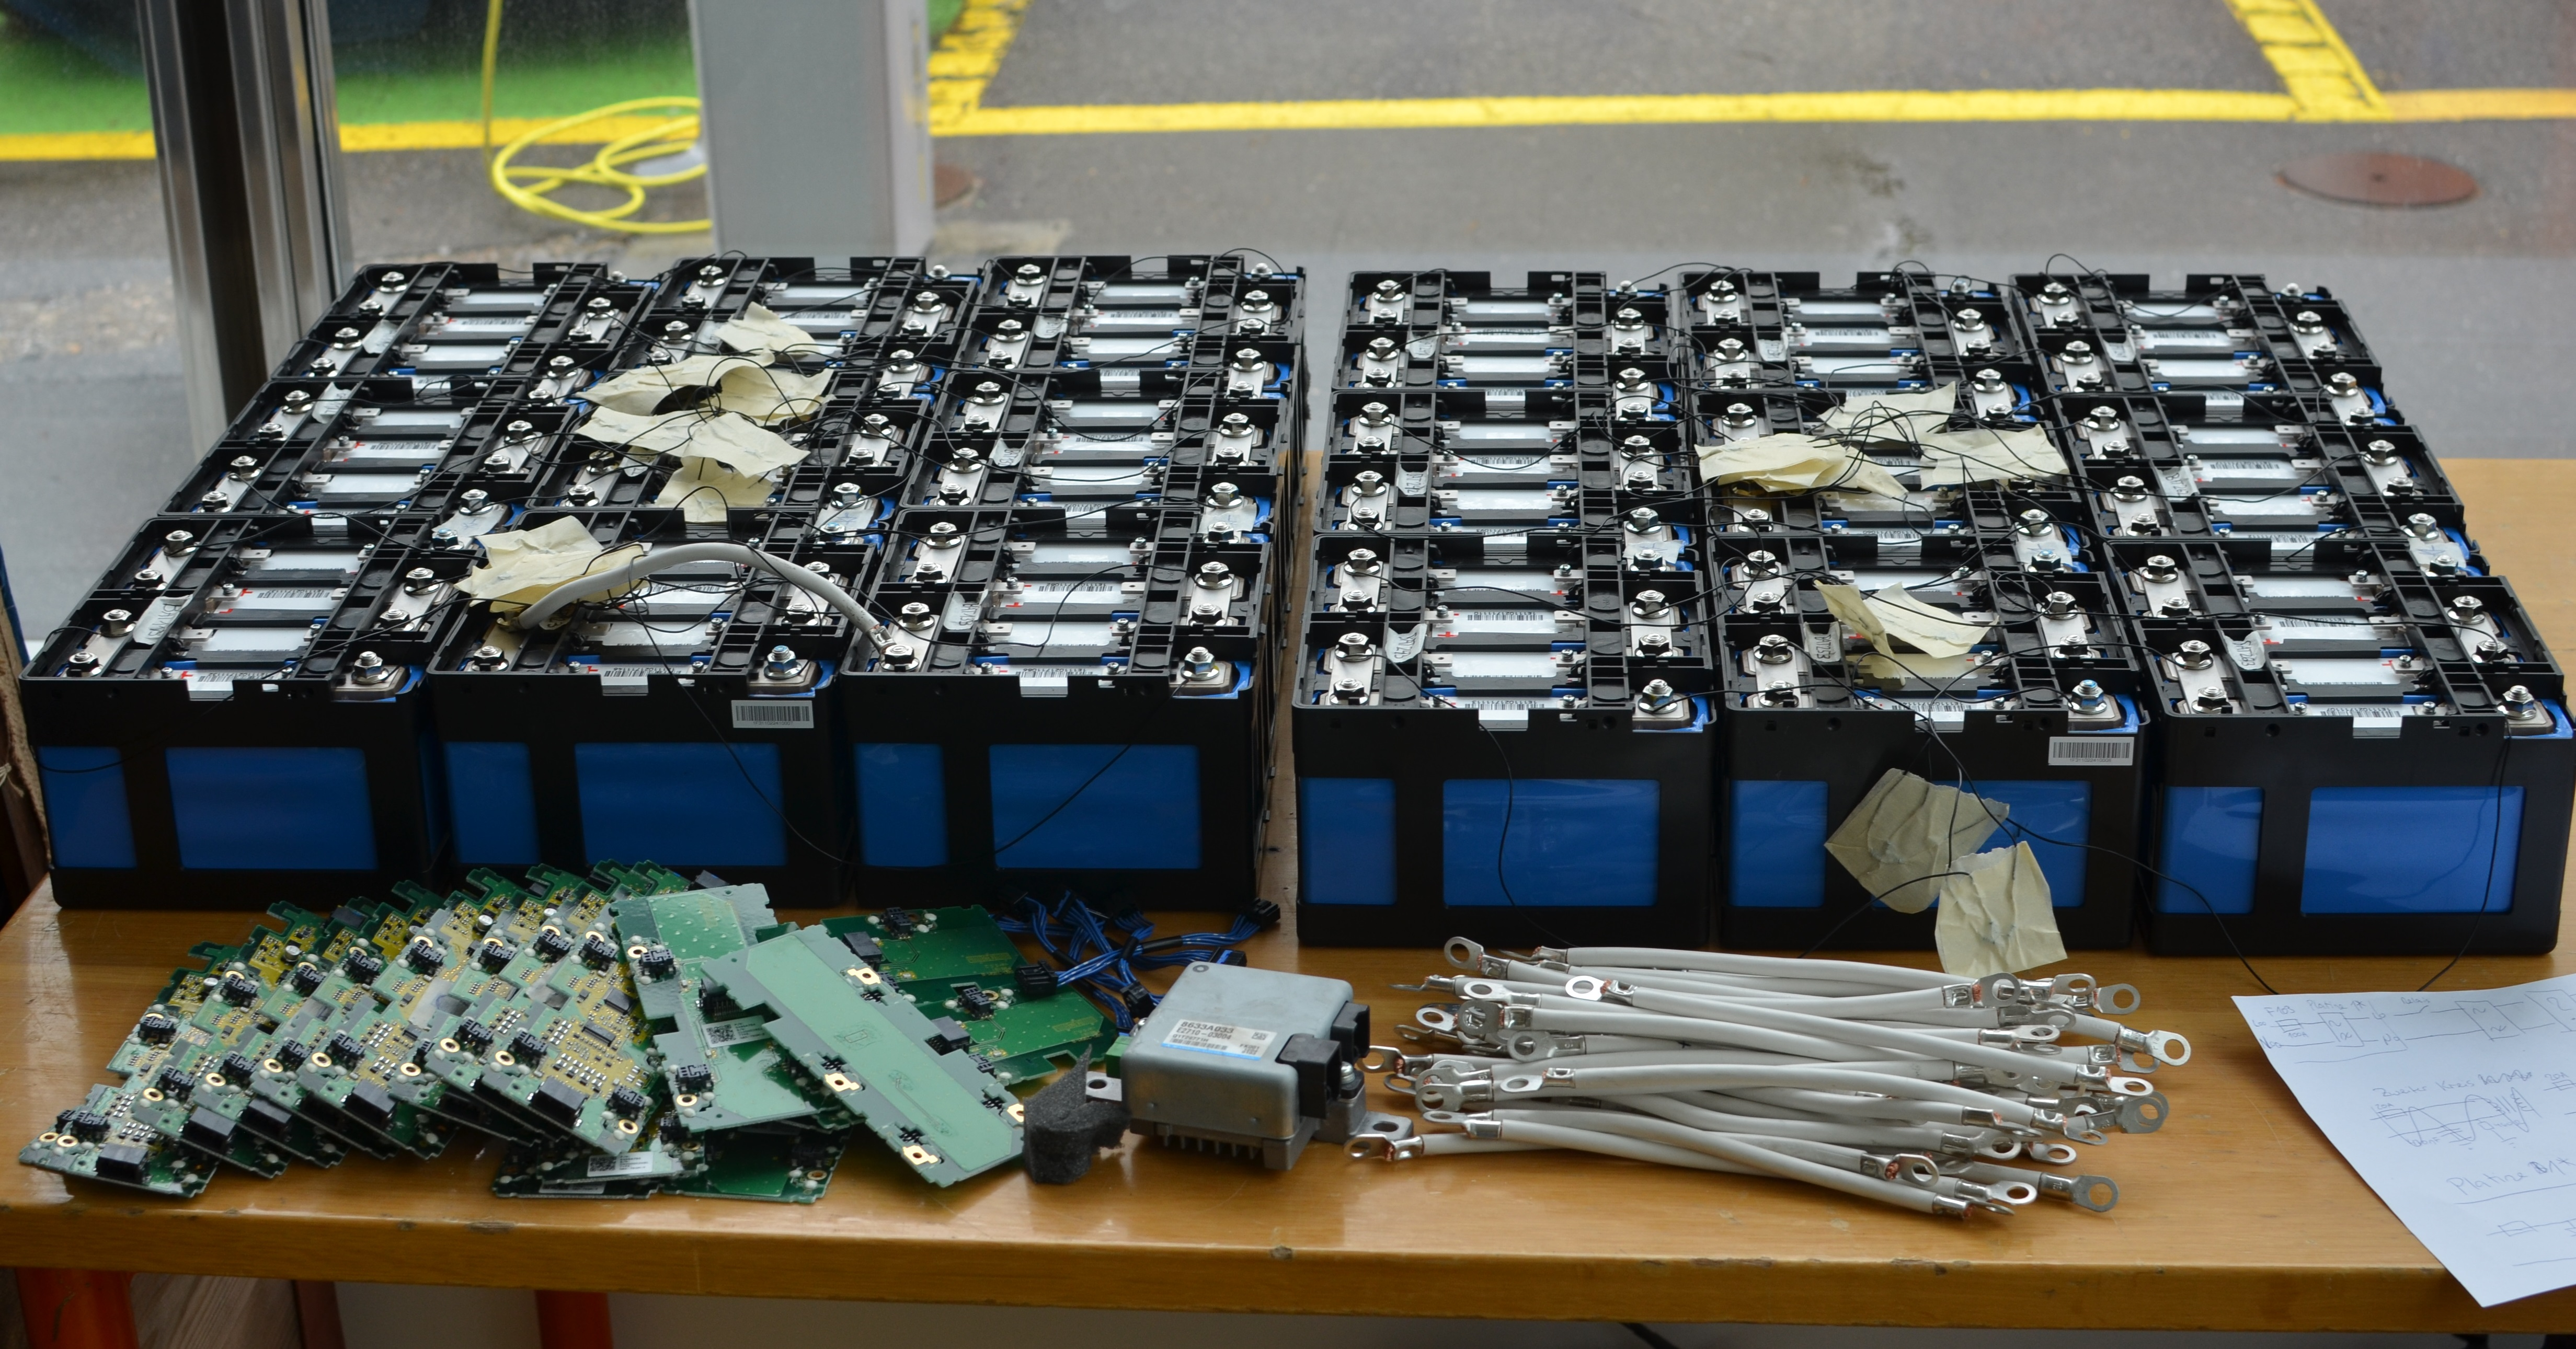
\includegraphics[width=1.3\textwidth]{images/Anhang/Batteriepakete.jpg}
	\caption{\textcolor{blue}{Die Batteriepakete im Aufbau, wie er später im Fahrzeug gefunden wird}}
	\label{fig:Batteriepakete}
\end{figure}
\begin{figure}[h]
	\centering
		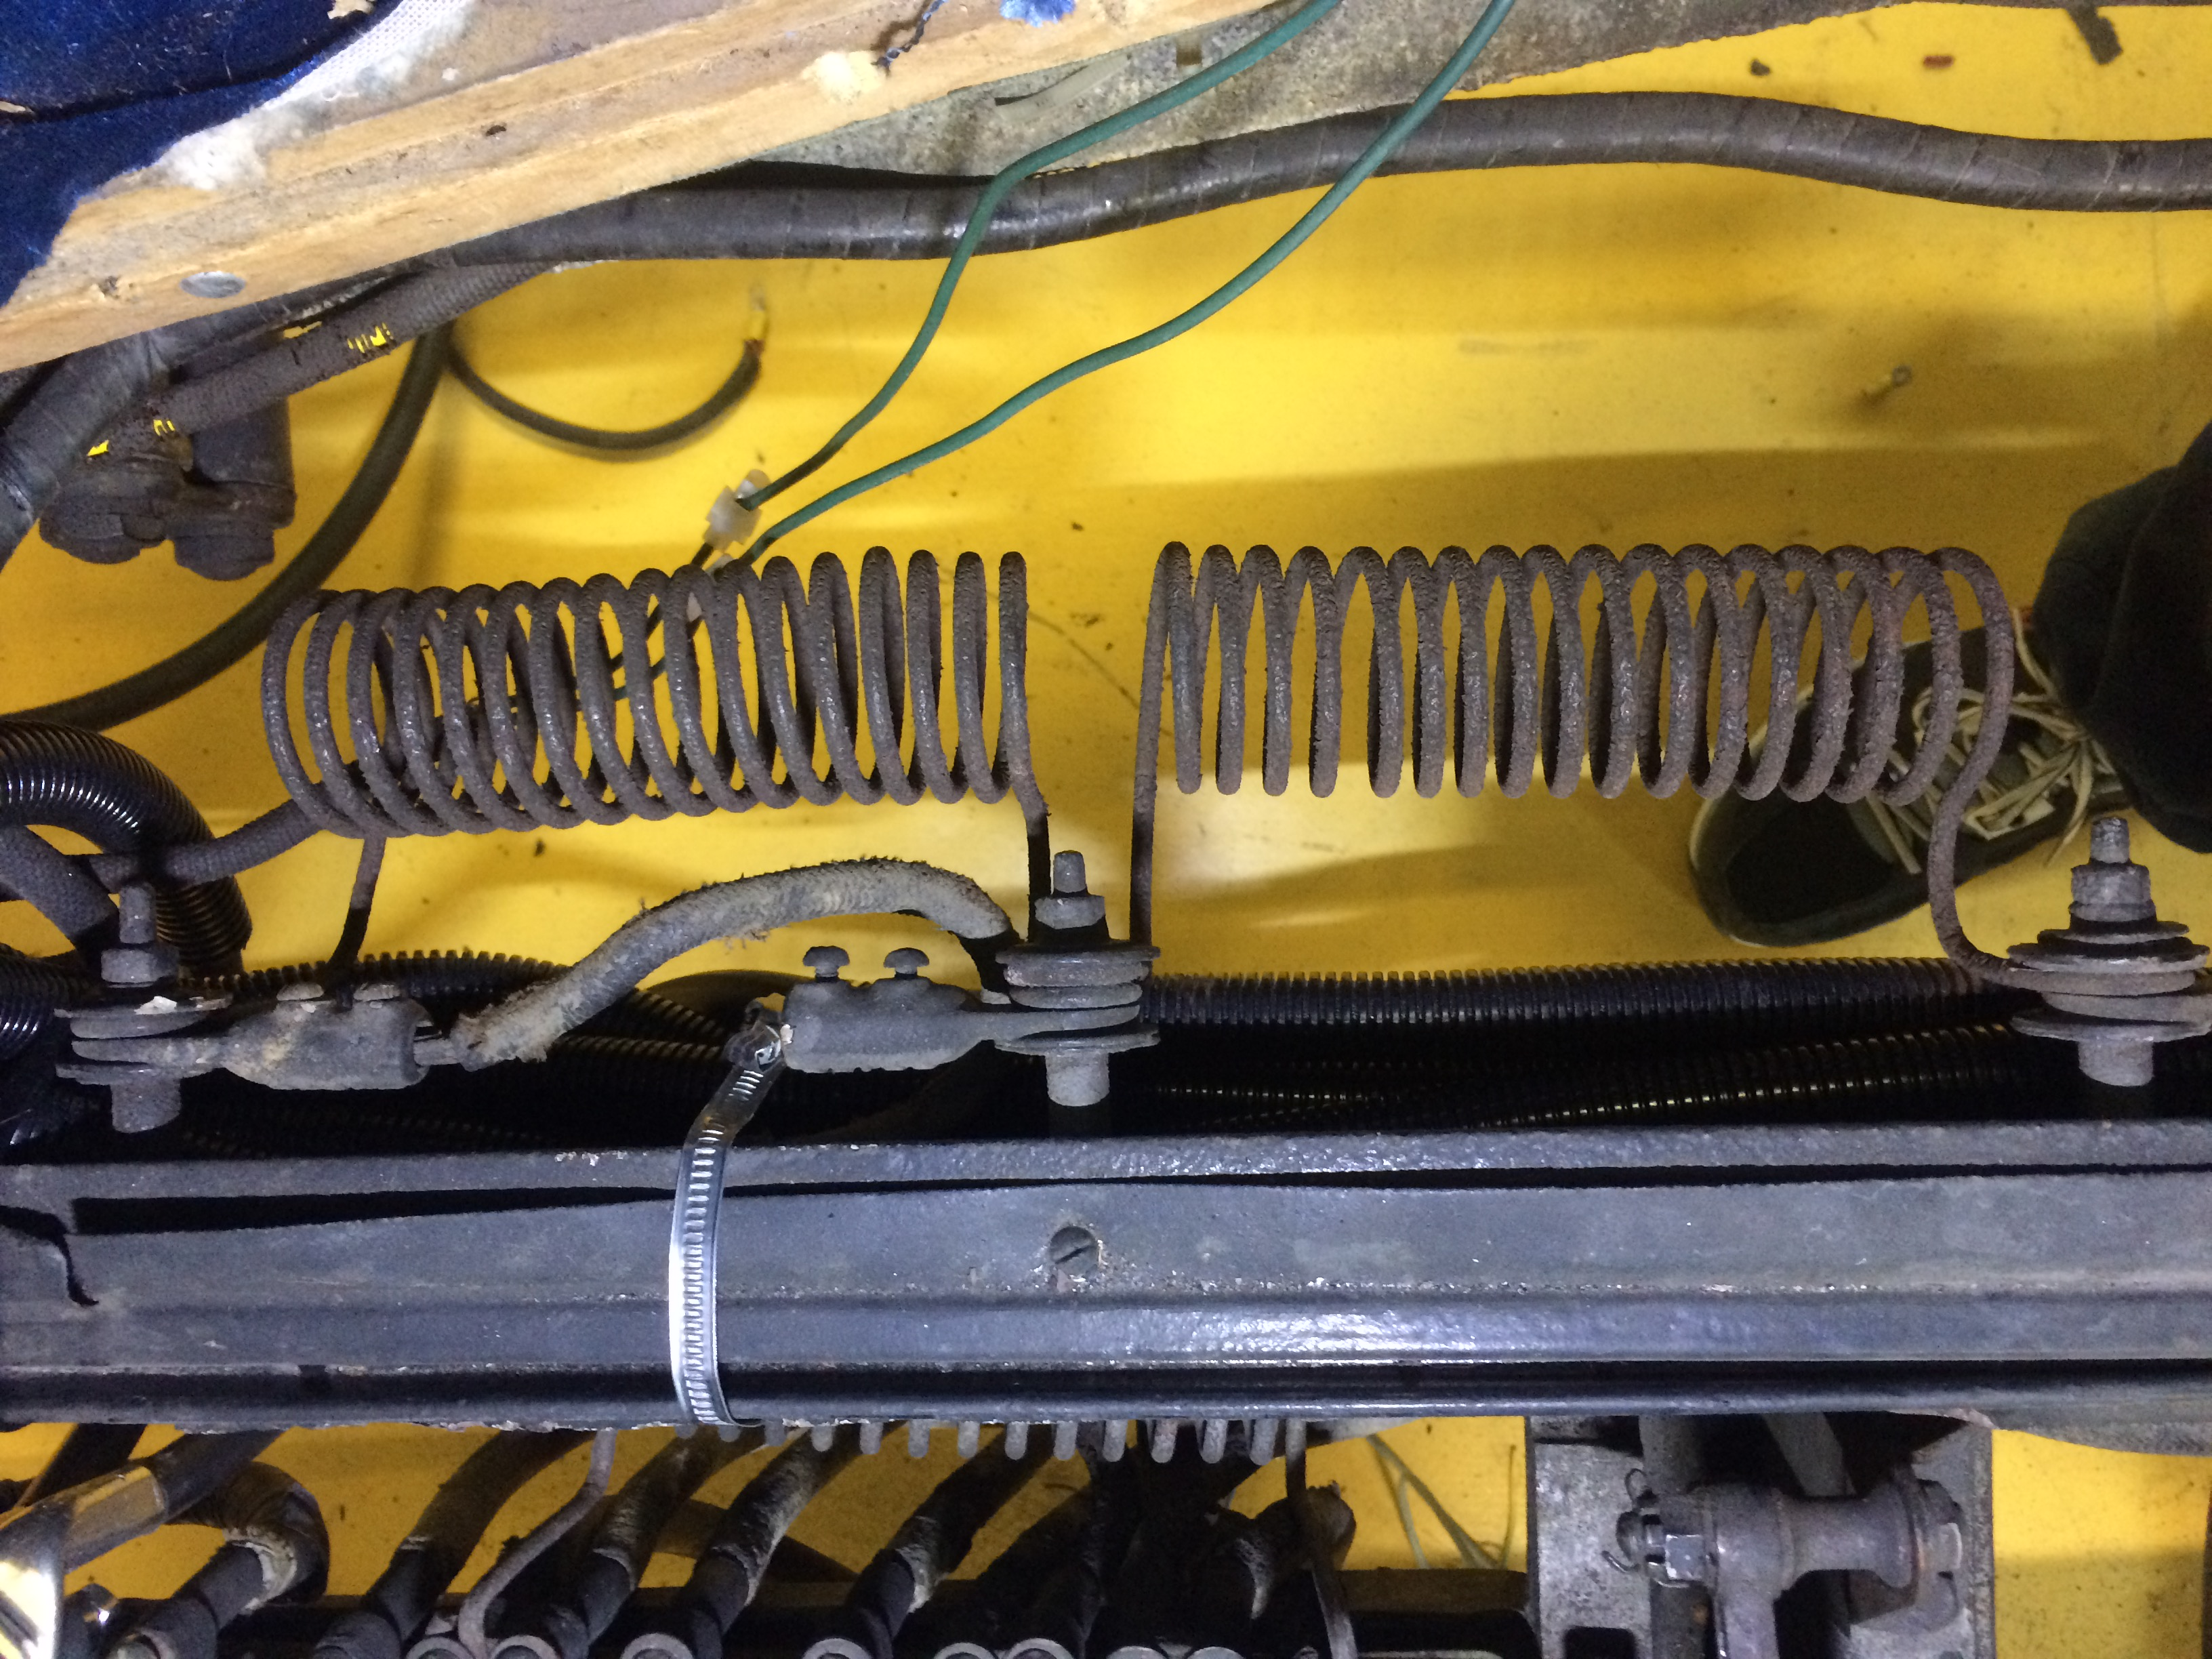
\includegraphics[angle=180,width=1.30\textwidth]{images/Anhang/Anfahrwiderstand.jpg}
	\caption{\textcolor{blue}{Der Anfahrwiderstand, in den Schemas als $R_1$ bezeichnet, befindet sich rechts neben dem Stufenschalter}}
	\label{fig:Anfahrwiderstand}
\end{figure}
\begin{figure}[h]
	\centering
		\includegraphics[width=1.30\textwidth]{images/Anhang/Cut-Out-Switch.jpg}
	\caption{\textcolor{blue}{Der Cut-Out-Switch unter dem Sitz vor dem Einbau des U-Stücks aus Kupfer, wobei man gut erkennt, wie die Kraft der Feder nicht ausreicht, um den Hebel vollständig in die Kontakte zu pressen}}
	\label{fig:Cut-Out-Switch}
\end{figure}
\begin{figure}[h]
	\centering
		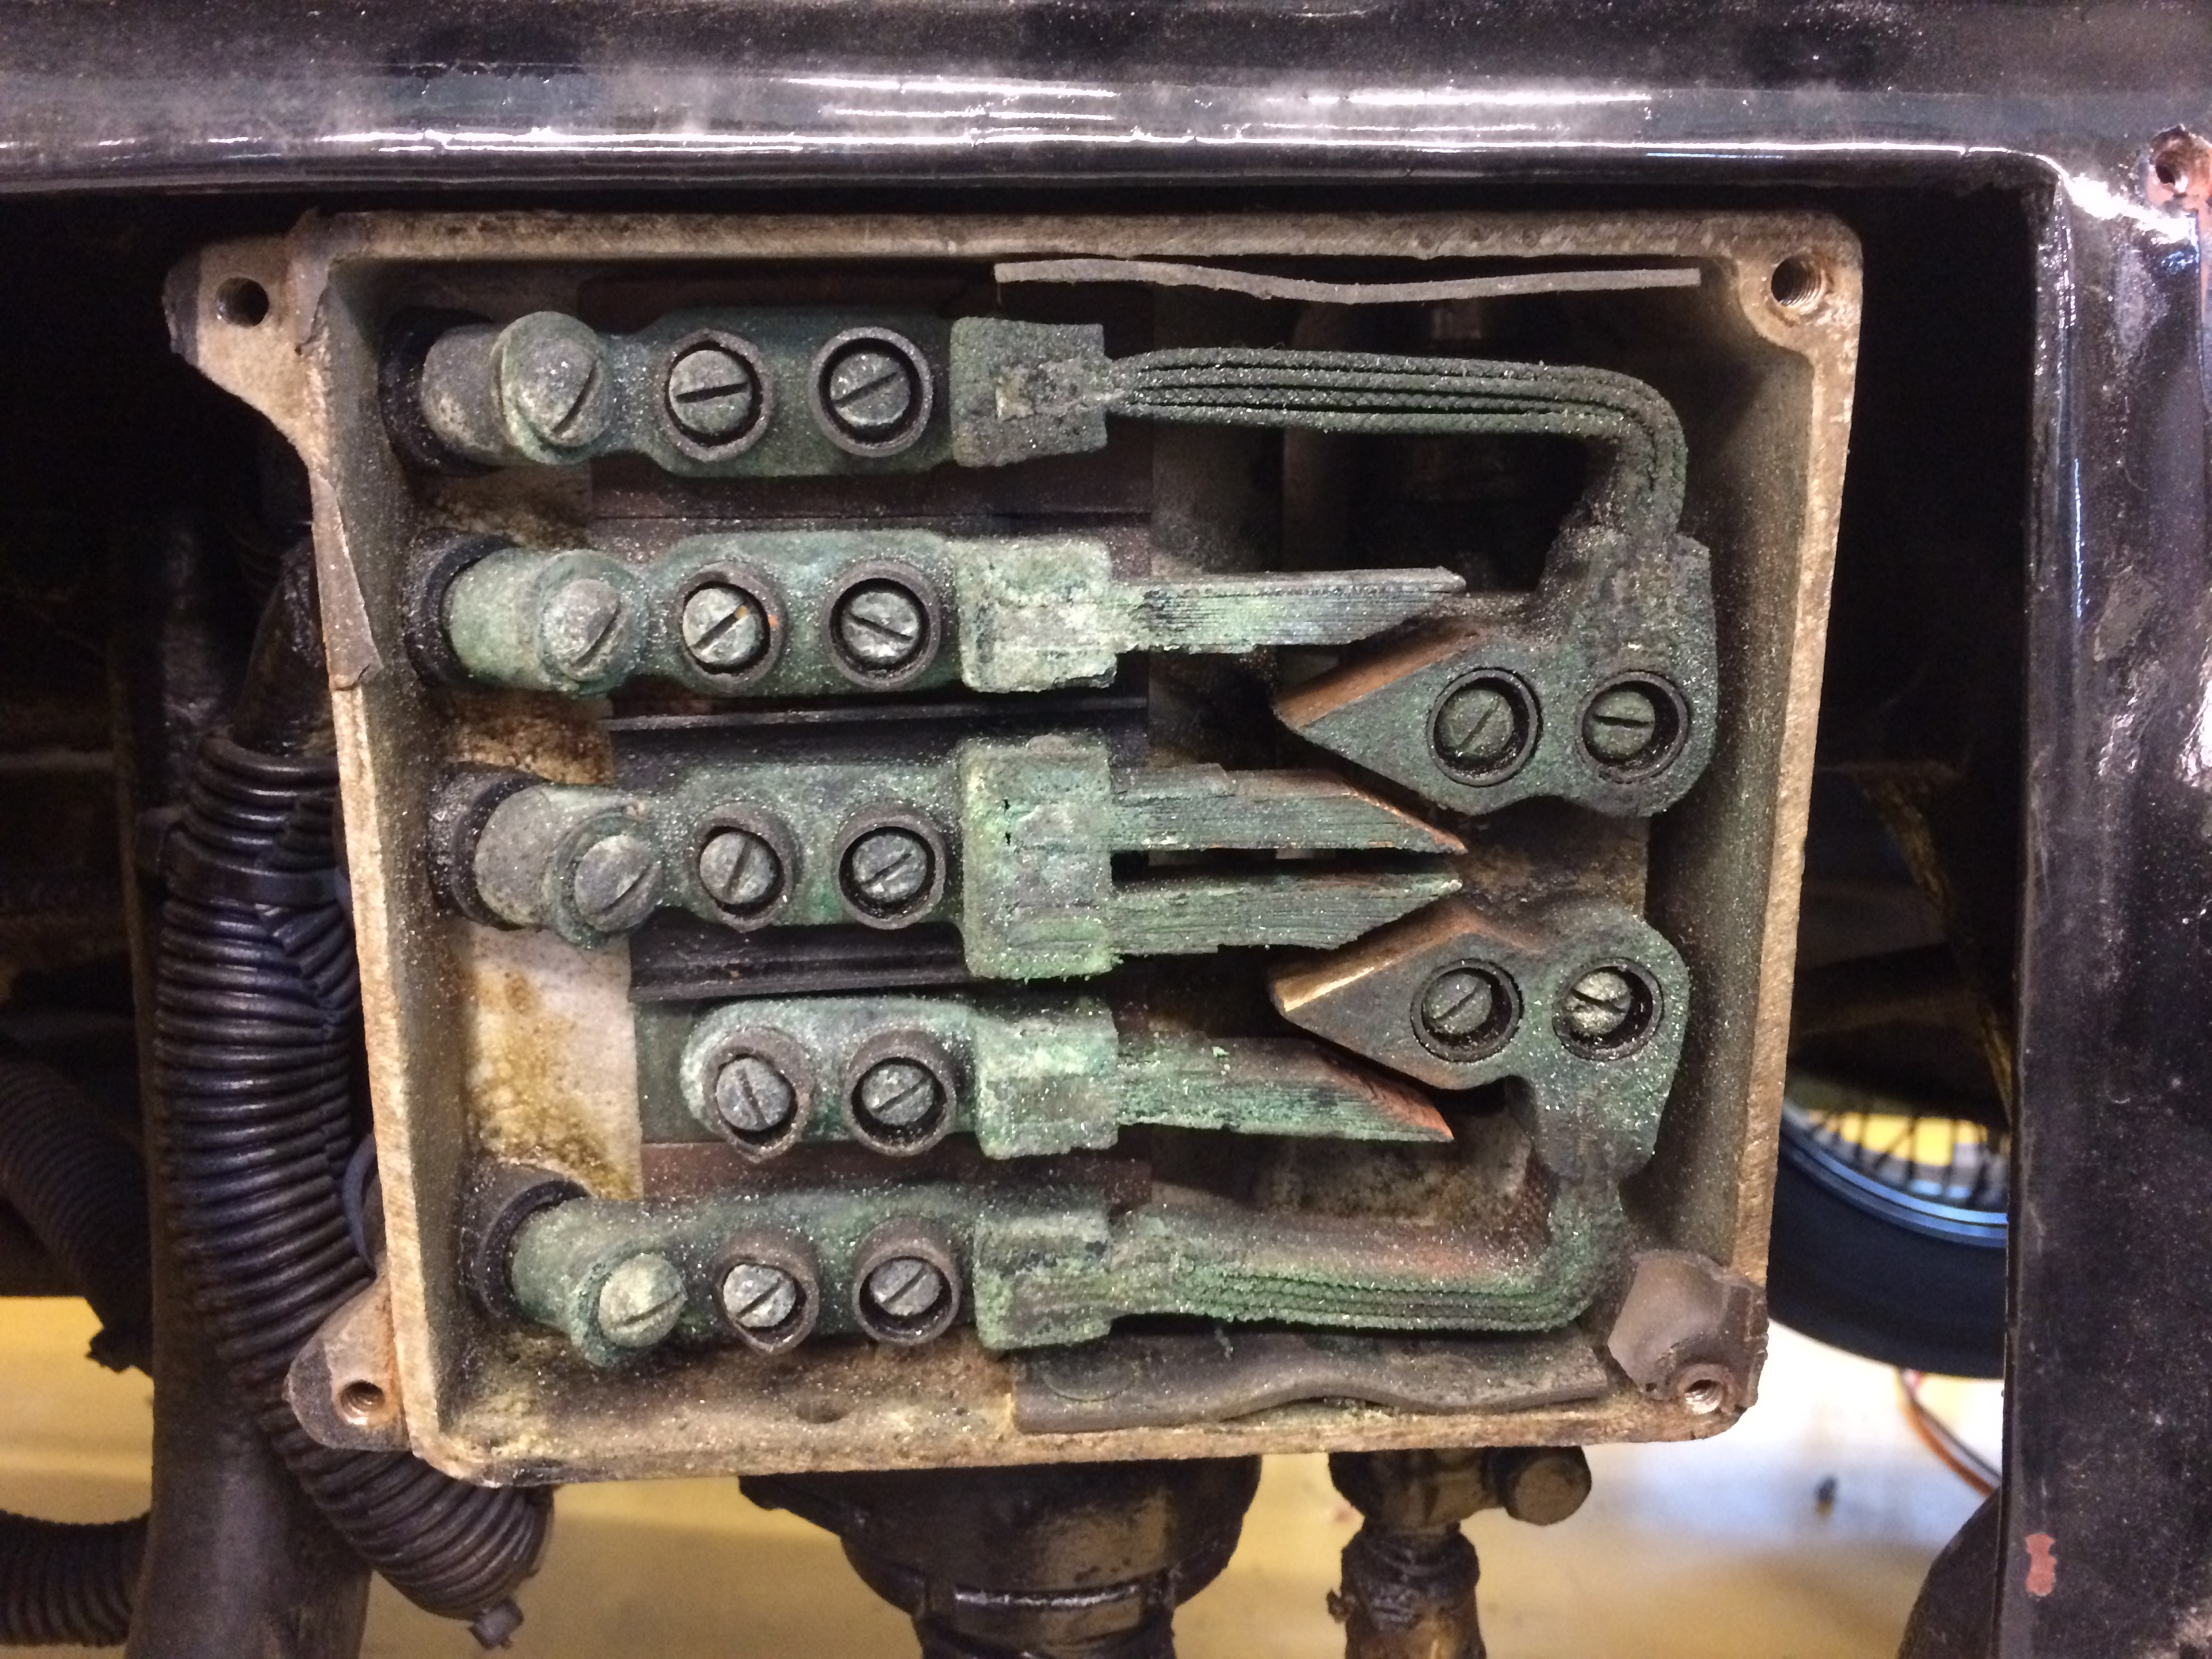
\includegraphics[width=1.30\textwidth]{images/Anhang/Fahrtrichtung.jpg}
	\caption{\textcolor{blue}{Die Auswahl der Fahrtrichtung erfolgt mit einem klassischen Polwendeschalter, wobei die beiden \grqq spitzen\grqq$~$ Kontakte rechts bewegt werden können}}
	\label{fig:Fahrtrichtung}
\end{figure}
\begin{figure}[h]
	\centering
		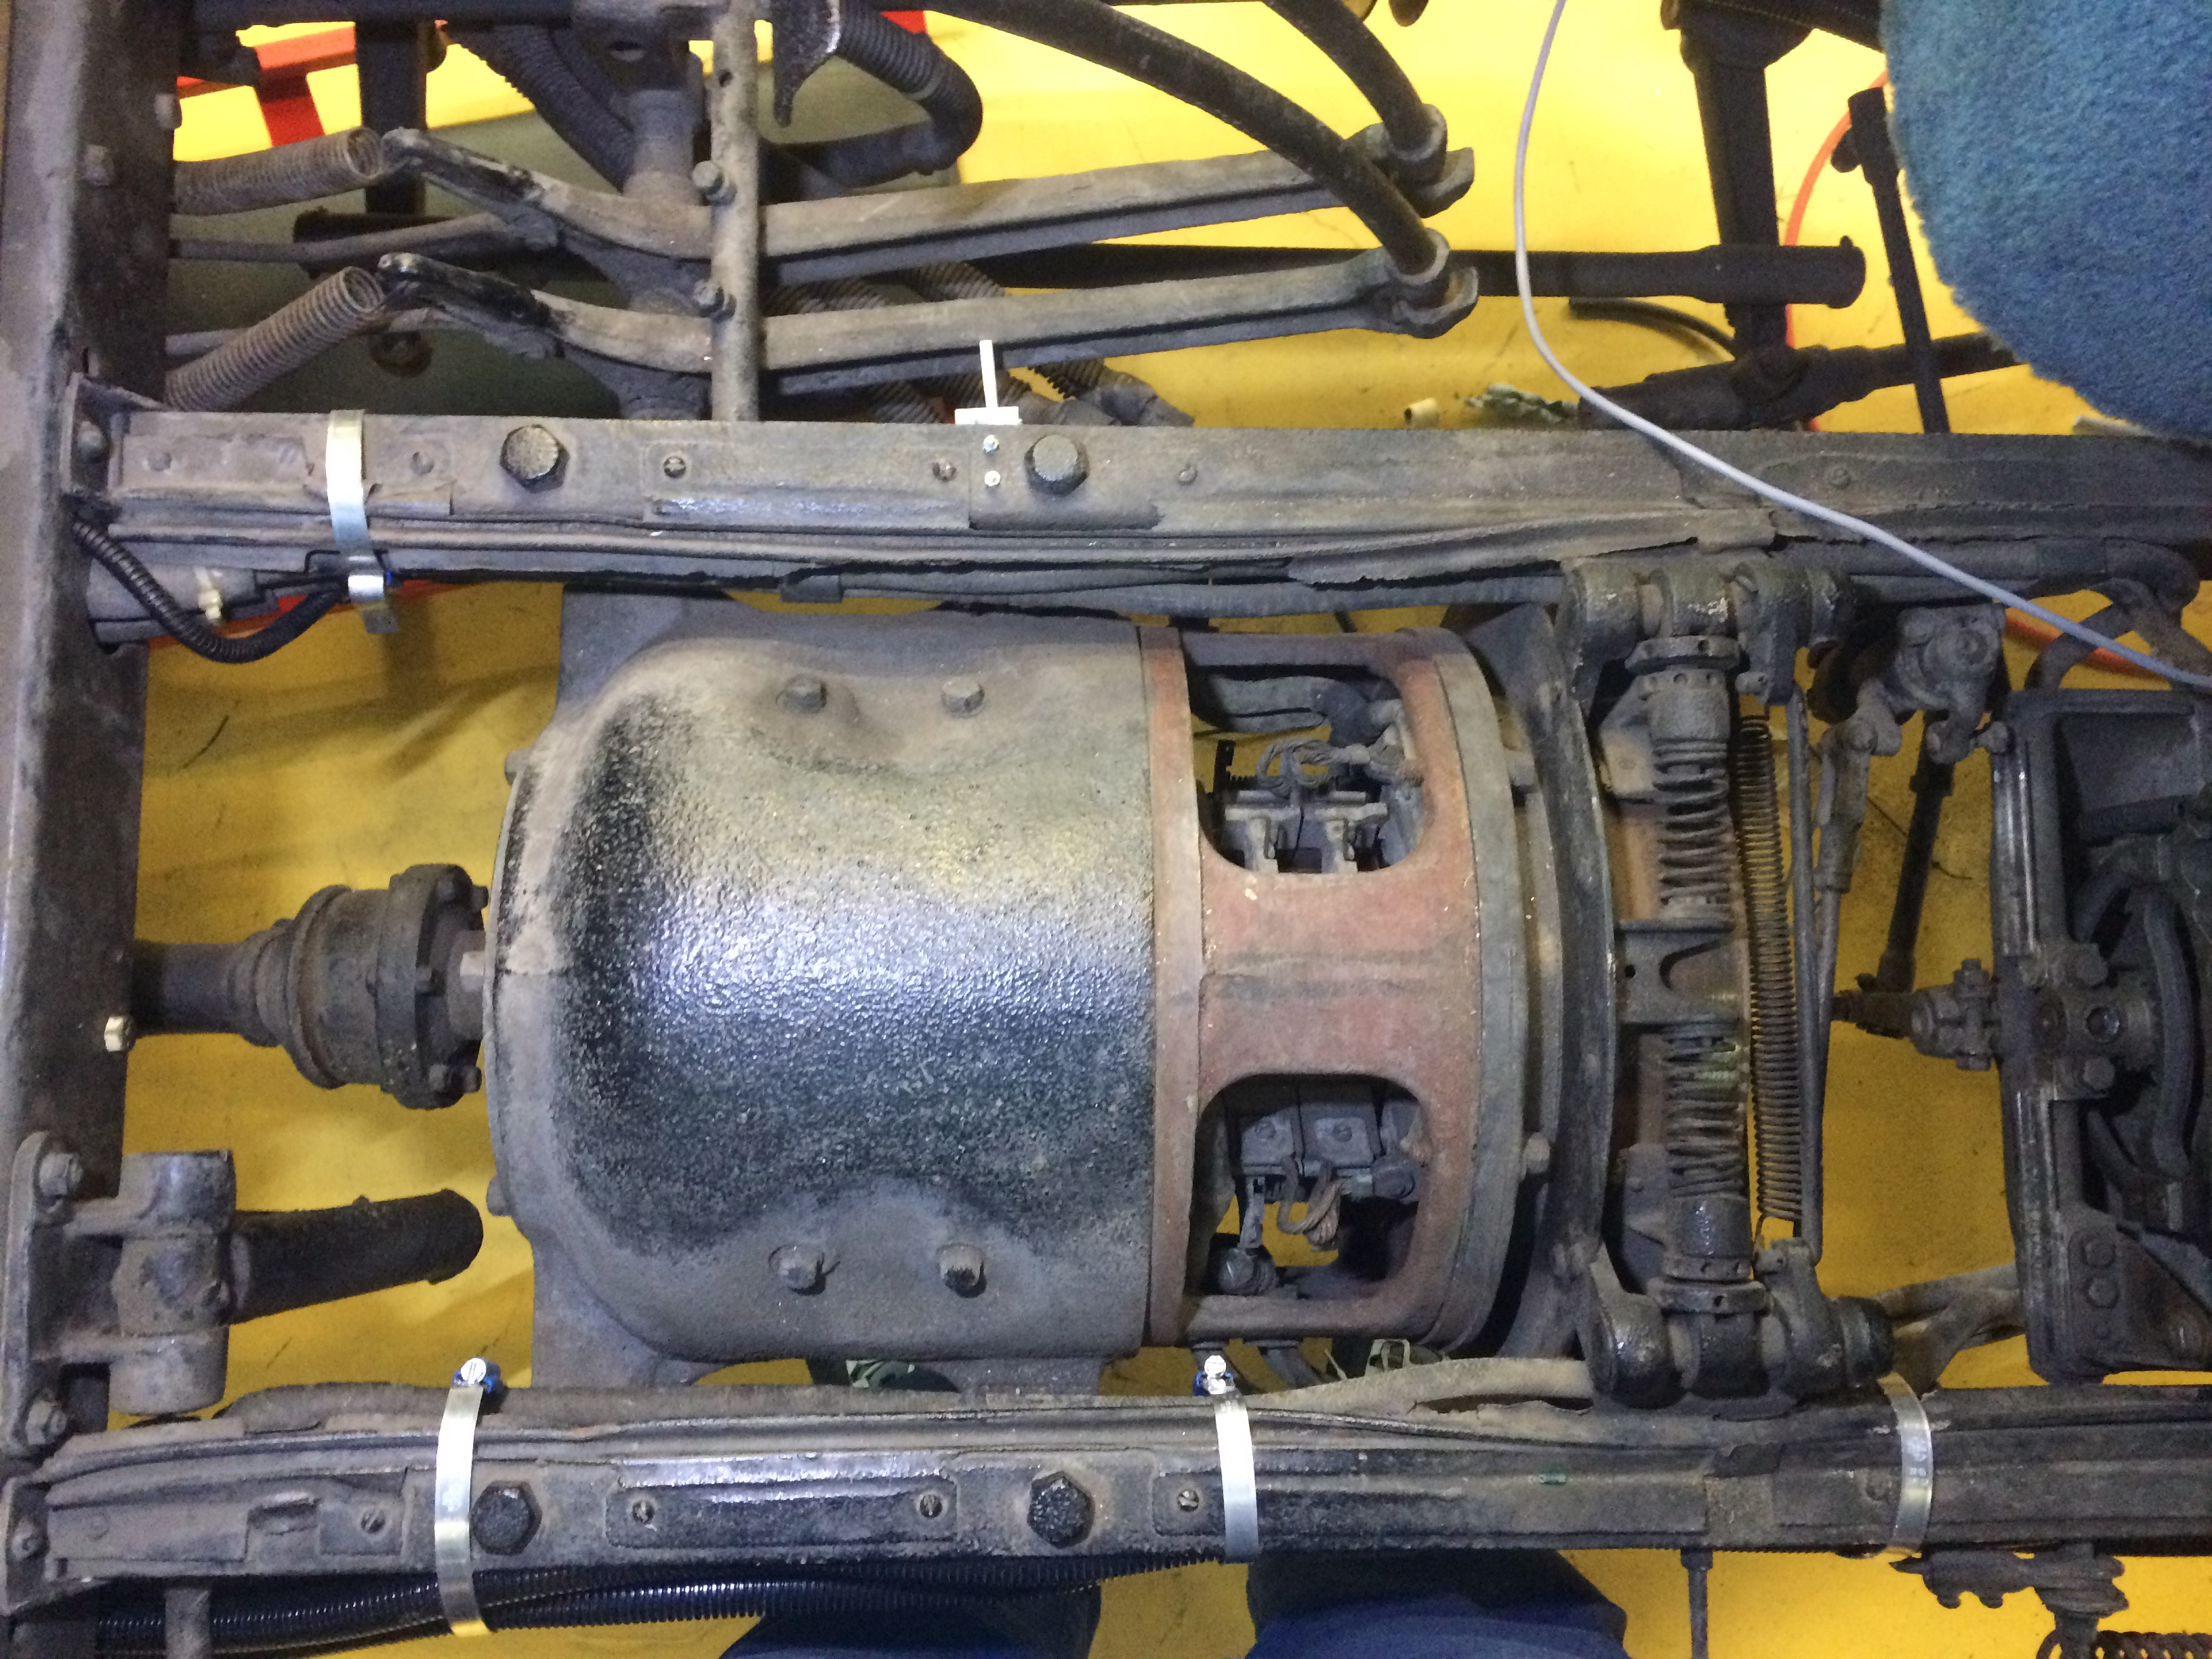
\includegraphics[angle=180,width=1.30\textwidth]{images/Anhang/Motor.jpg}
	\caption{\textcolor{blue}{Blick von oben auf den Gleichstrom-Reihenschlussmotor, welcher eine Leistung von ungefähr $4.5$ PS aufweist ($3.3$ kW)}}
	\label{fig:Motor}
\end{figure}
\begin{figure}[h]
	\centering
		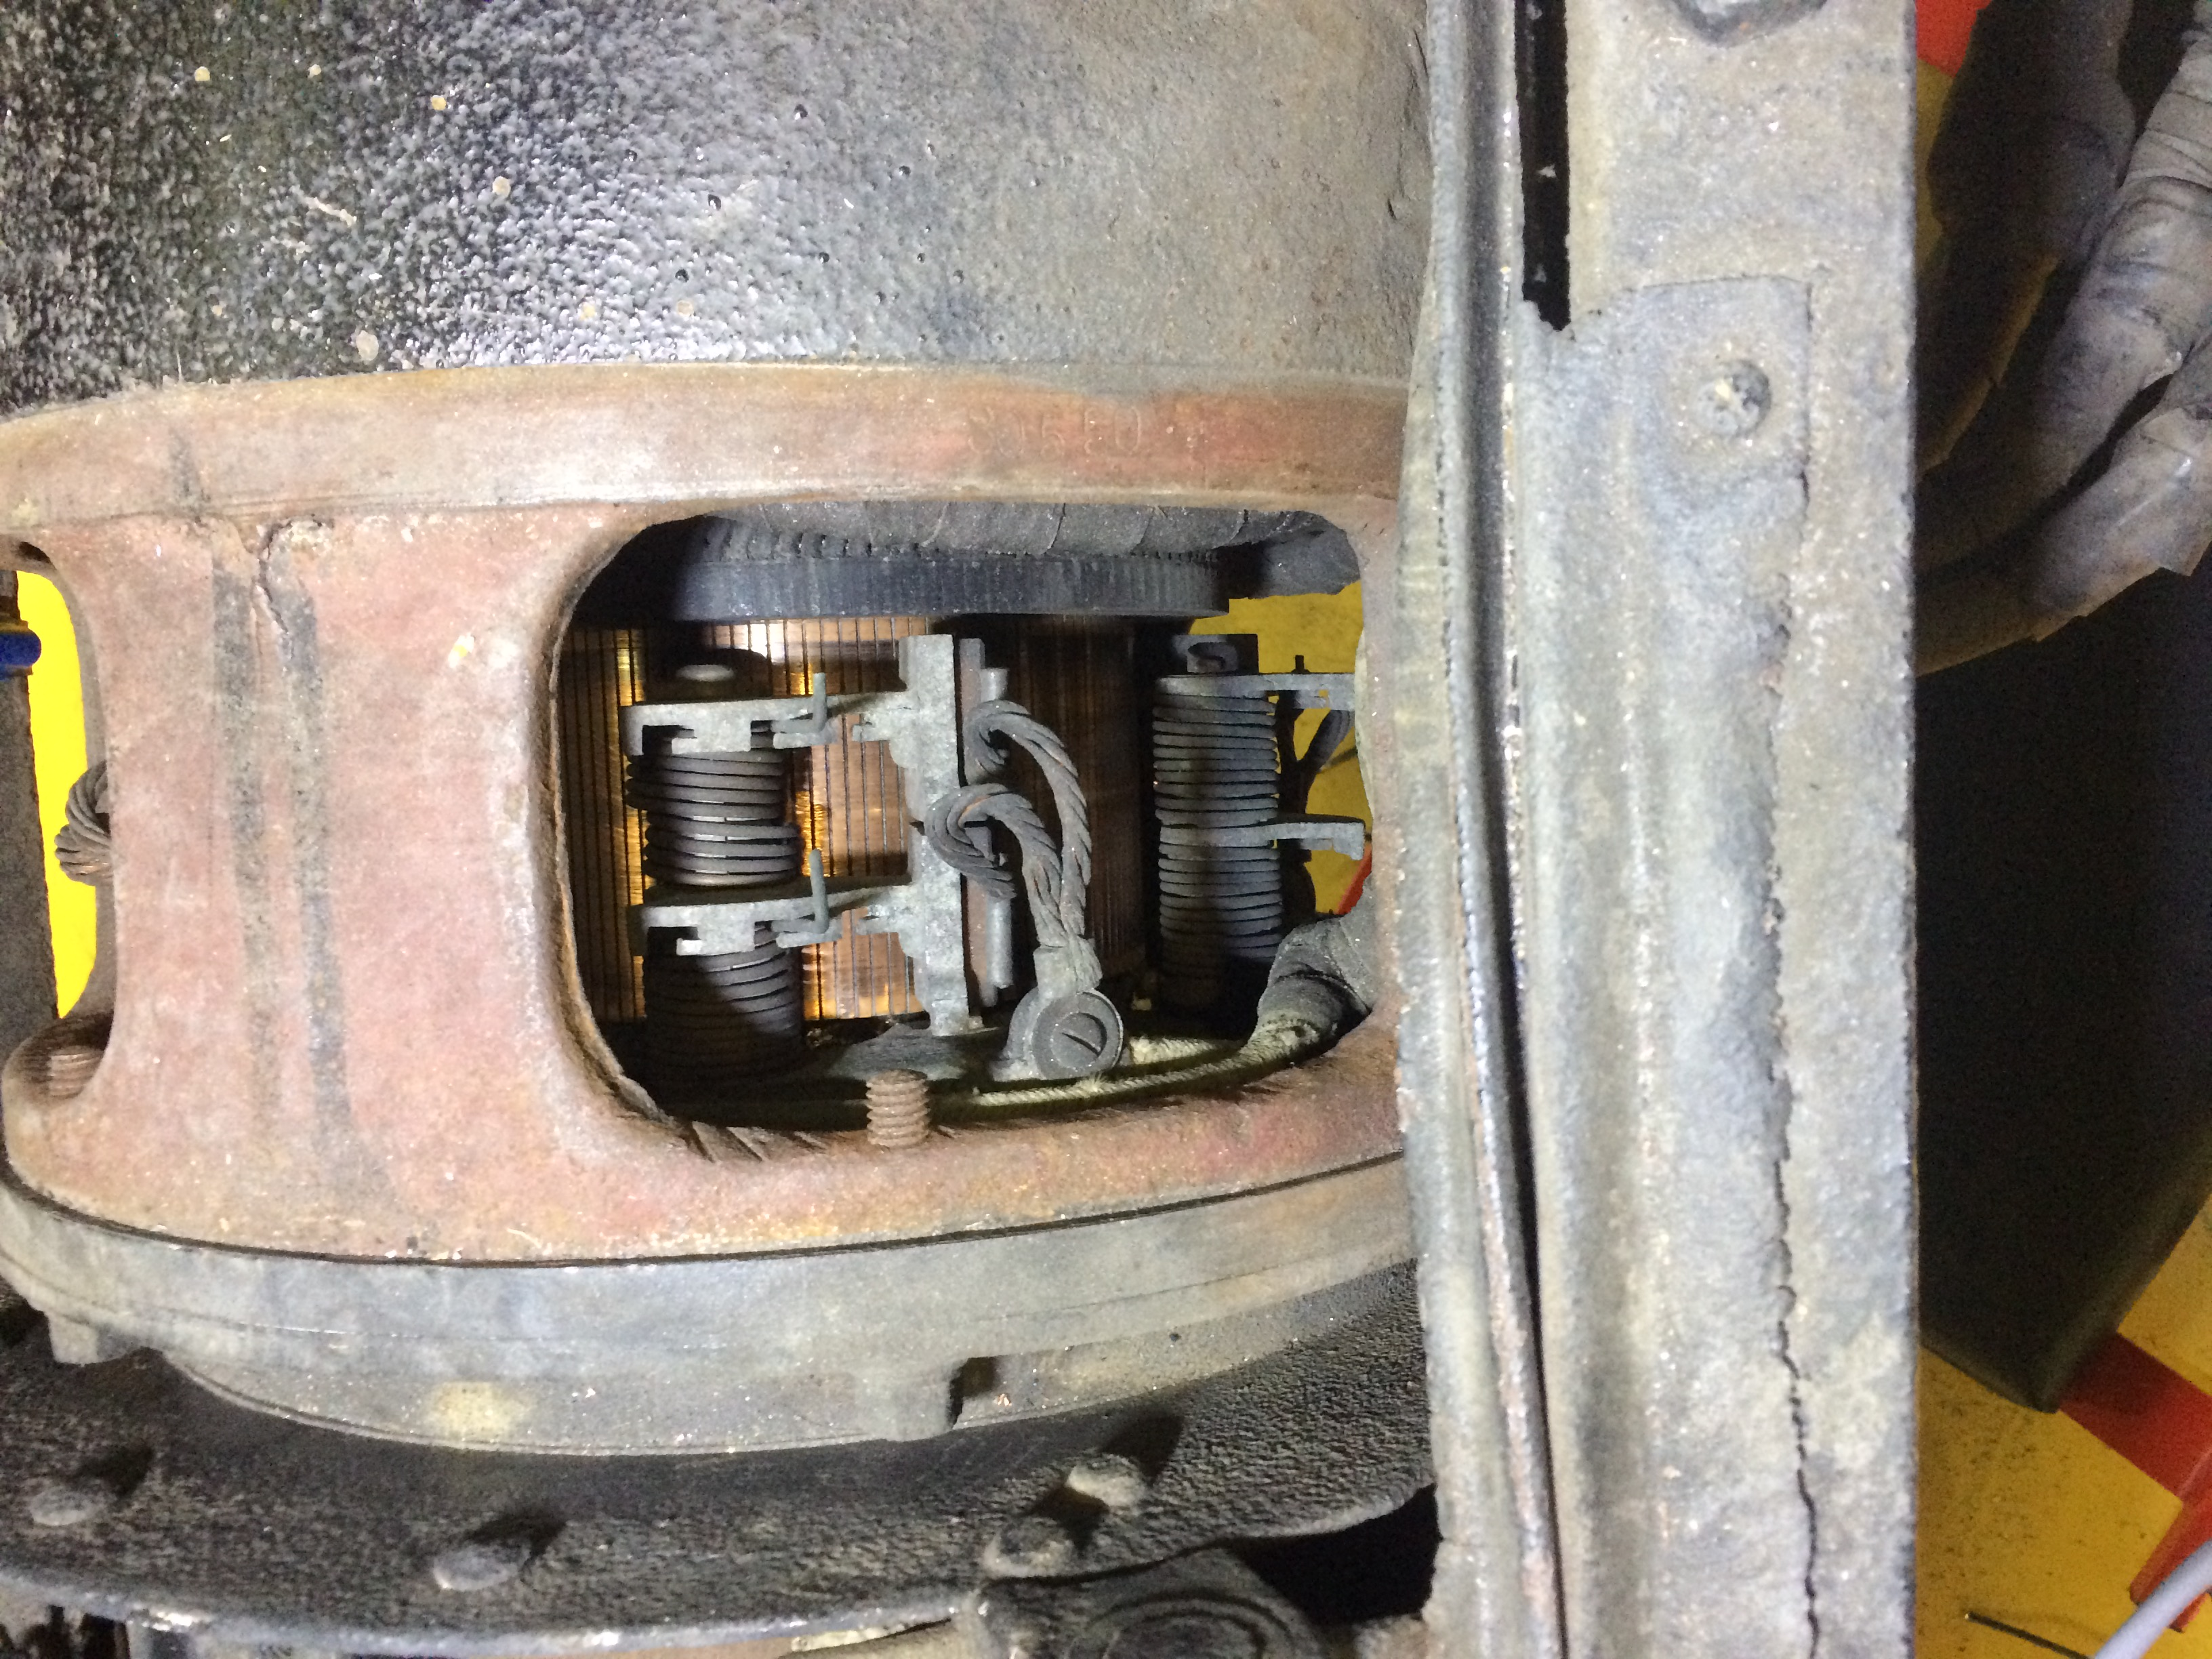
\includegraphics[angle=180,width=1.30\textwidth]{images/Anhang/Kollektor.jpg}
	\caption{\textcolor{blue}{Detailbetrachtung des Kollektors, welcher sehr fein ausgeführt ist}}
	\label{fig:Kollektor_Anhang}
\end{figure}
\begin{figure}[h]
	\centering
		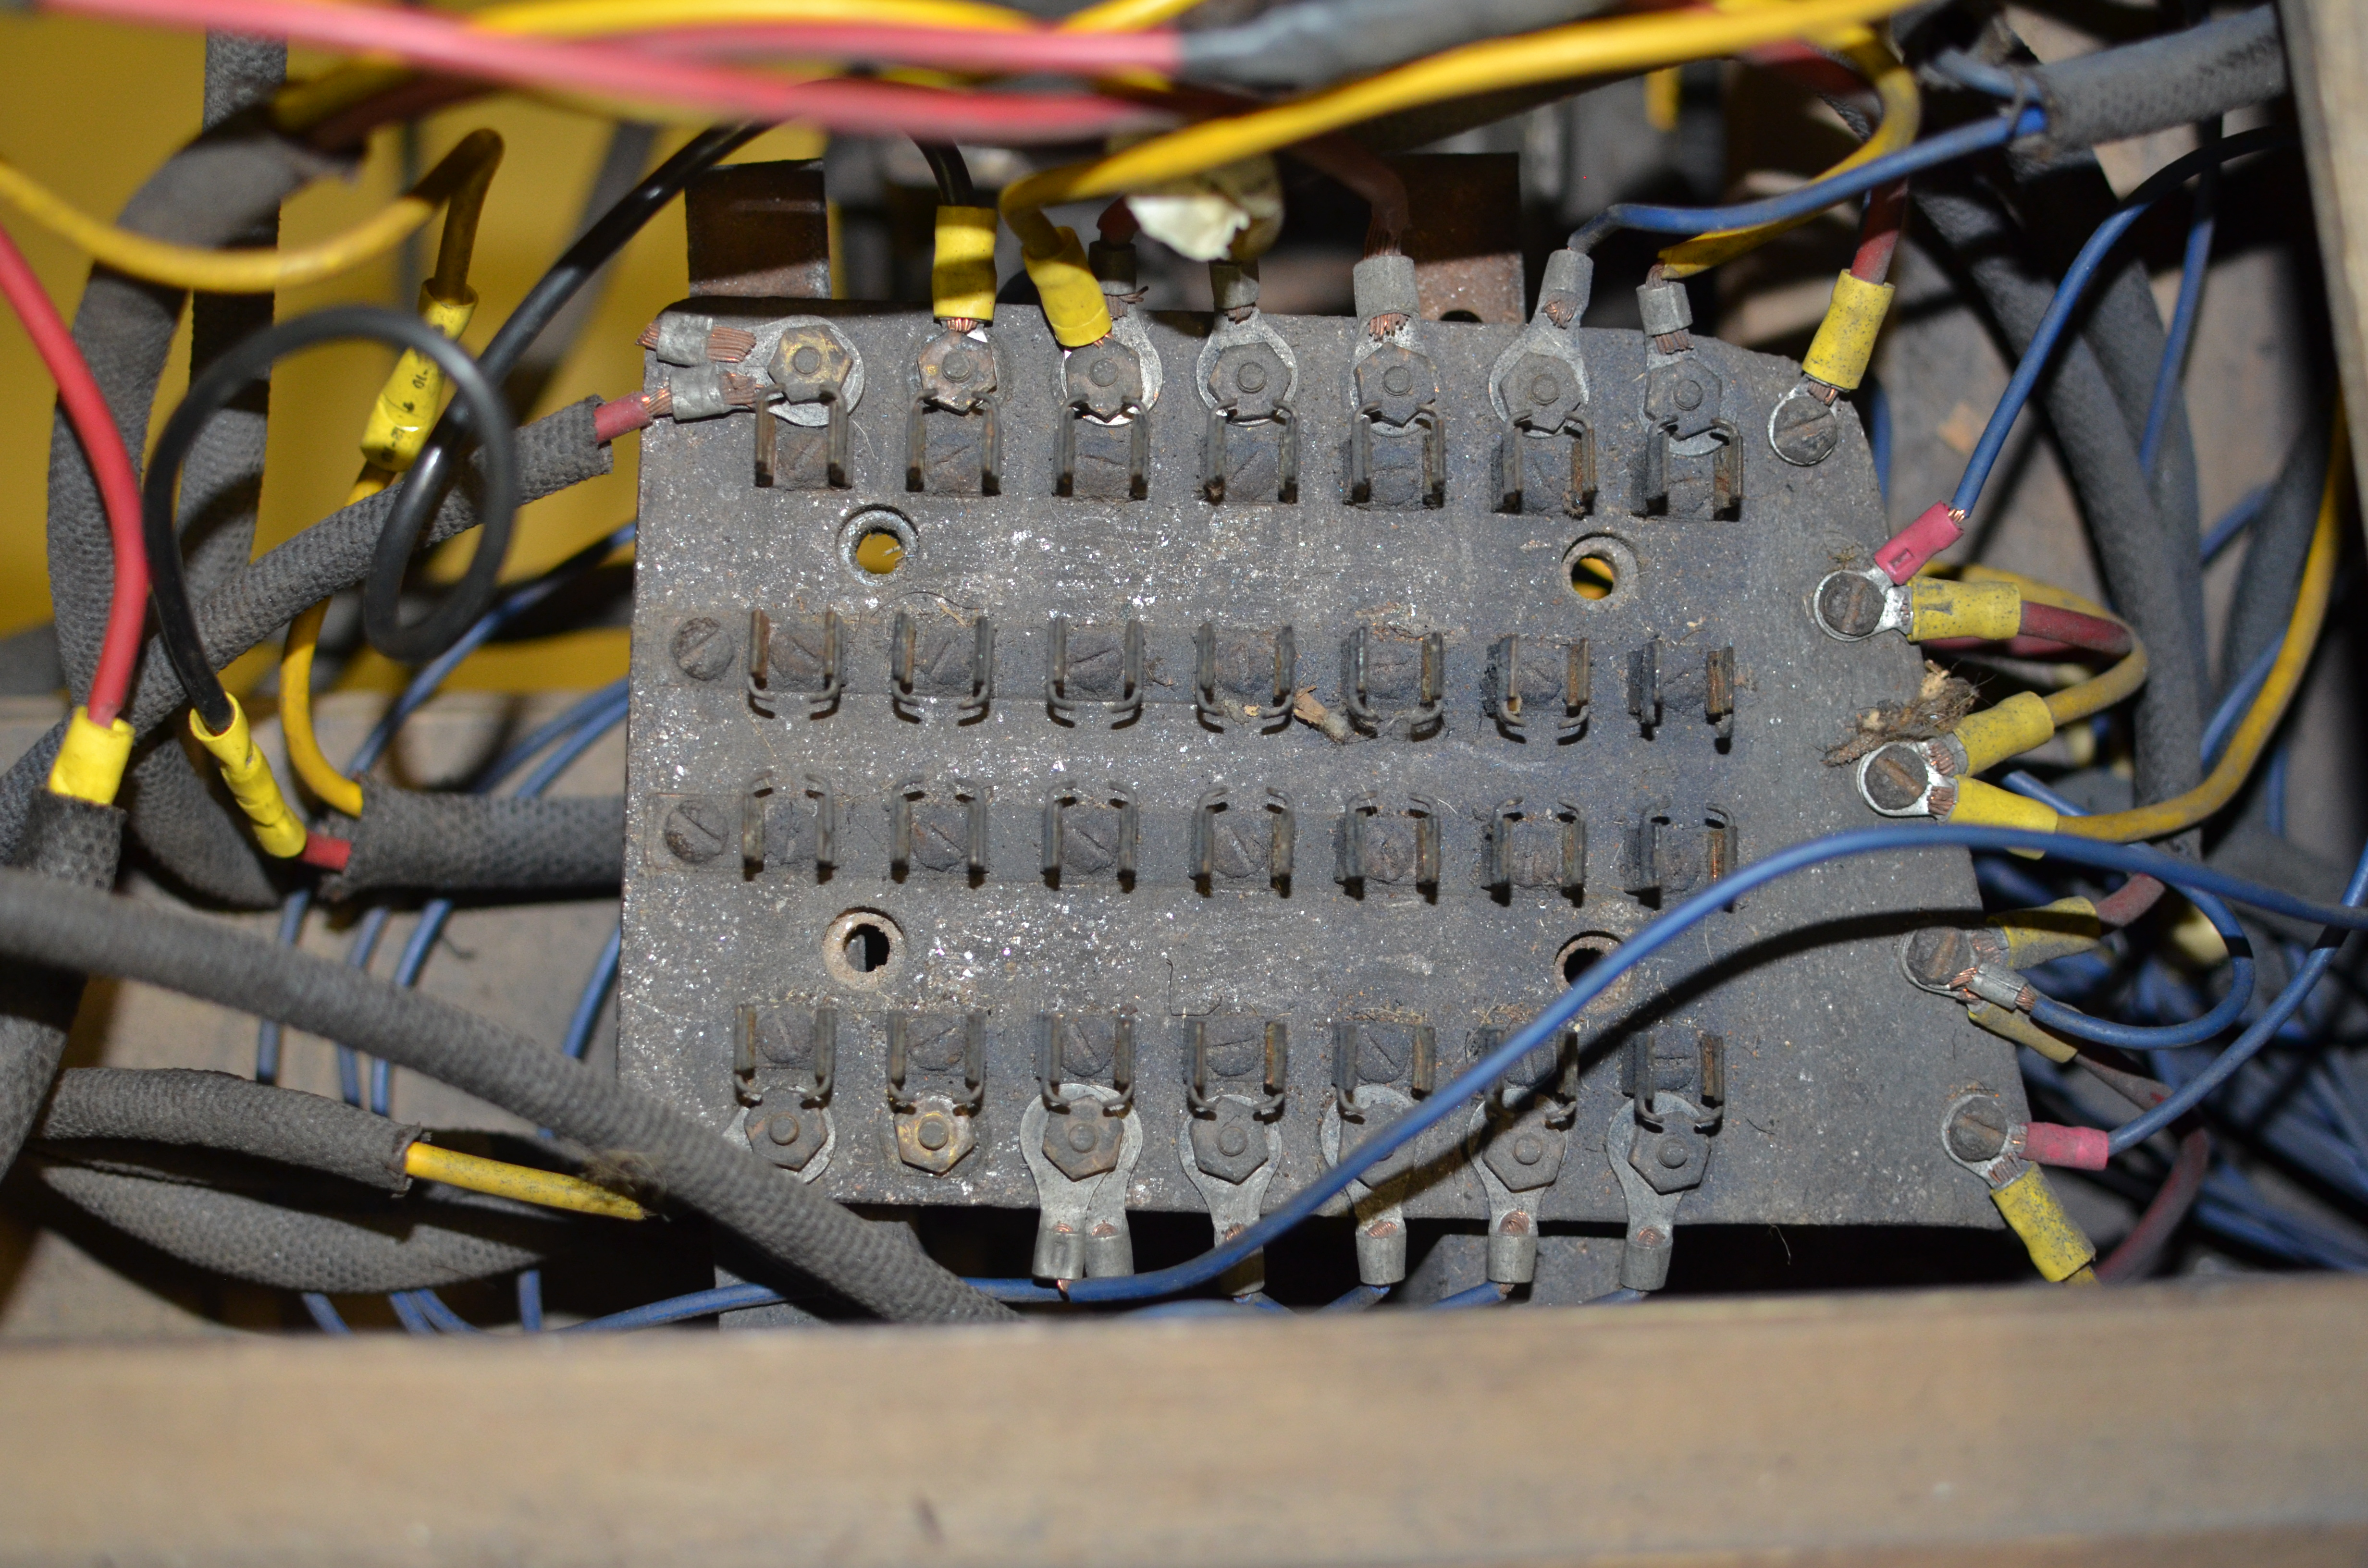
\includegraphics[width=1.30\textwidth]{images/Anhang/Sicherungsbrett_Beleuchtung.jpg}
	\caption{\textcolor{blue}{Das Sicherungsbrett für die Beleuchtung, interessant ist hierbei, dass für beide Pole eine Sicherung vorhanden ist, was annehmen lässt, dass das Gehäuse des ursprünglichen Fahrzeugs in einer Mittelpunktspannung geerdet war}}
	\label{fig:Sicherungsbrett_Beleuchtung}
\end{figure}
\begin{figure}[h]
	\centering
		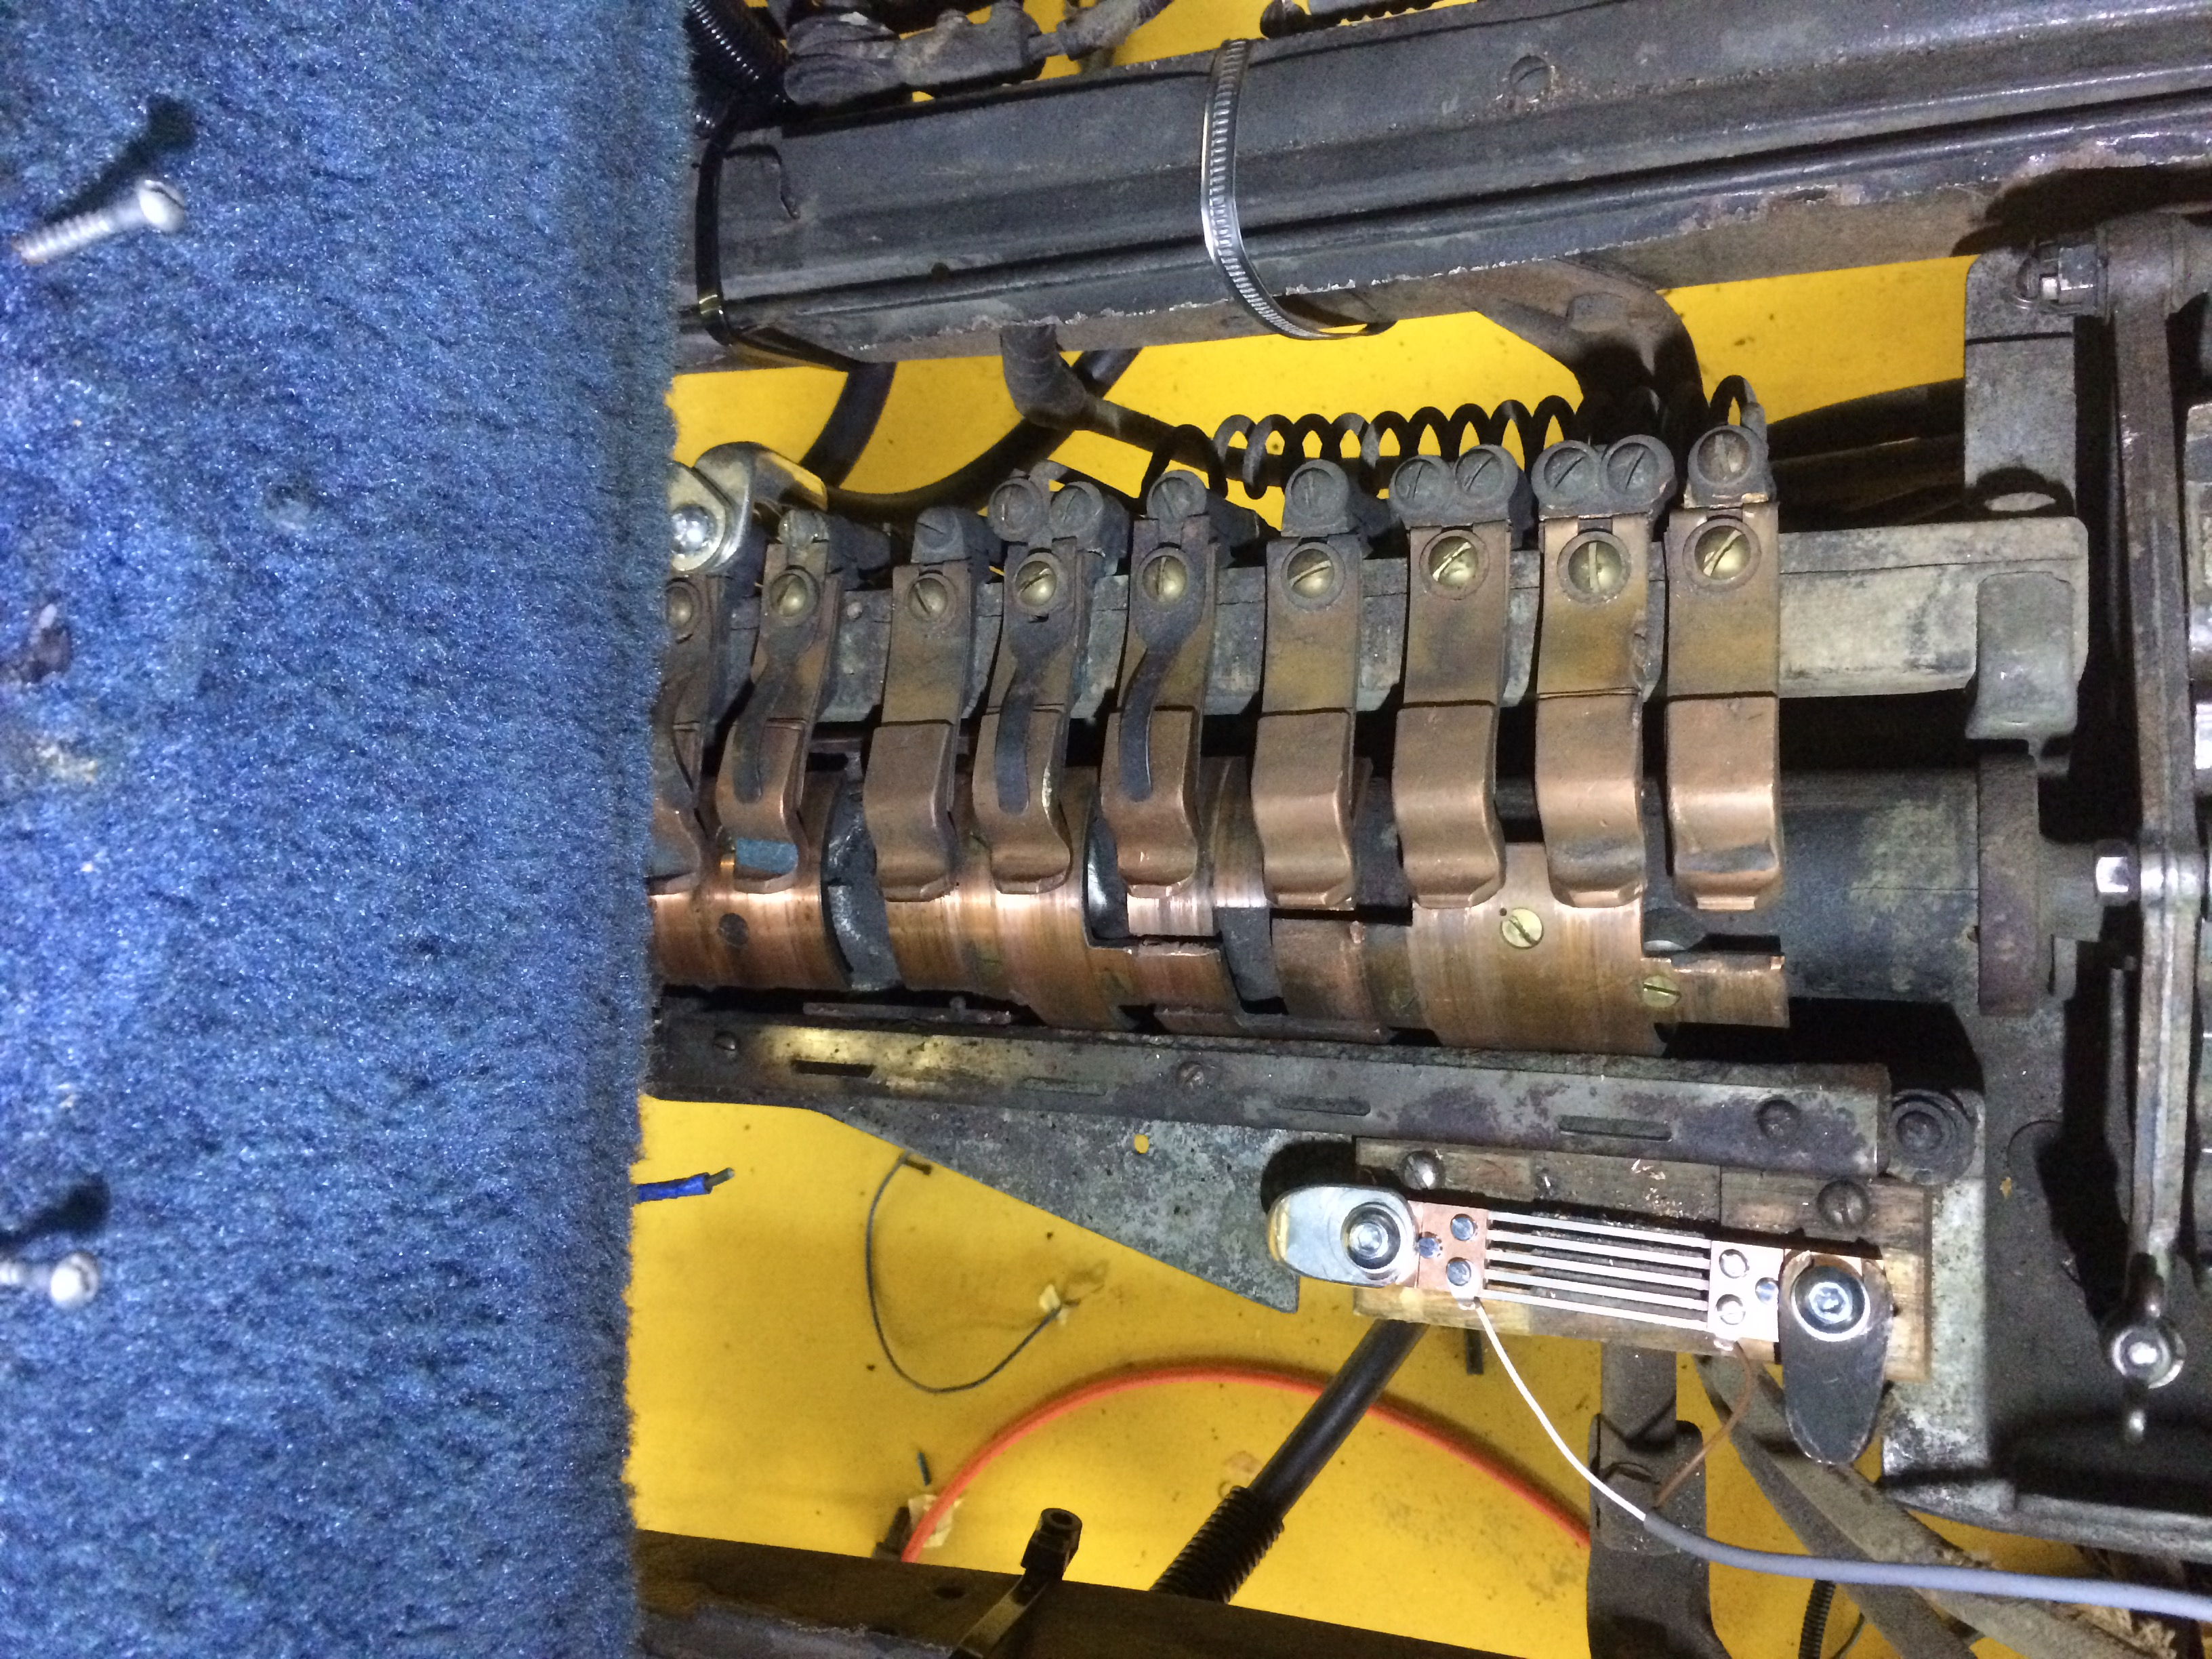
\includegraphics[width=1.30\textwidth]{images/Anhang/Stufenschalter.jpg}
	\caption{\textcolor{blue}{Der Stufenschalter mit den Kontaktfingern und Kontaktplatten, wobei ebenfalls der neue Shunt zu erkennen ist}}
	\label{fig:Stufenschalter_Anhang}
\end{figure}
\begin{figure}[h]
	\centering
		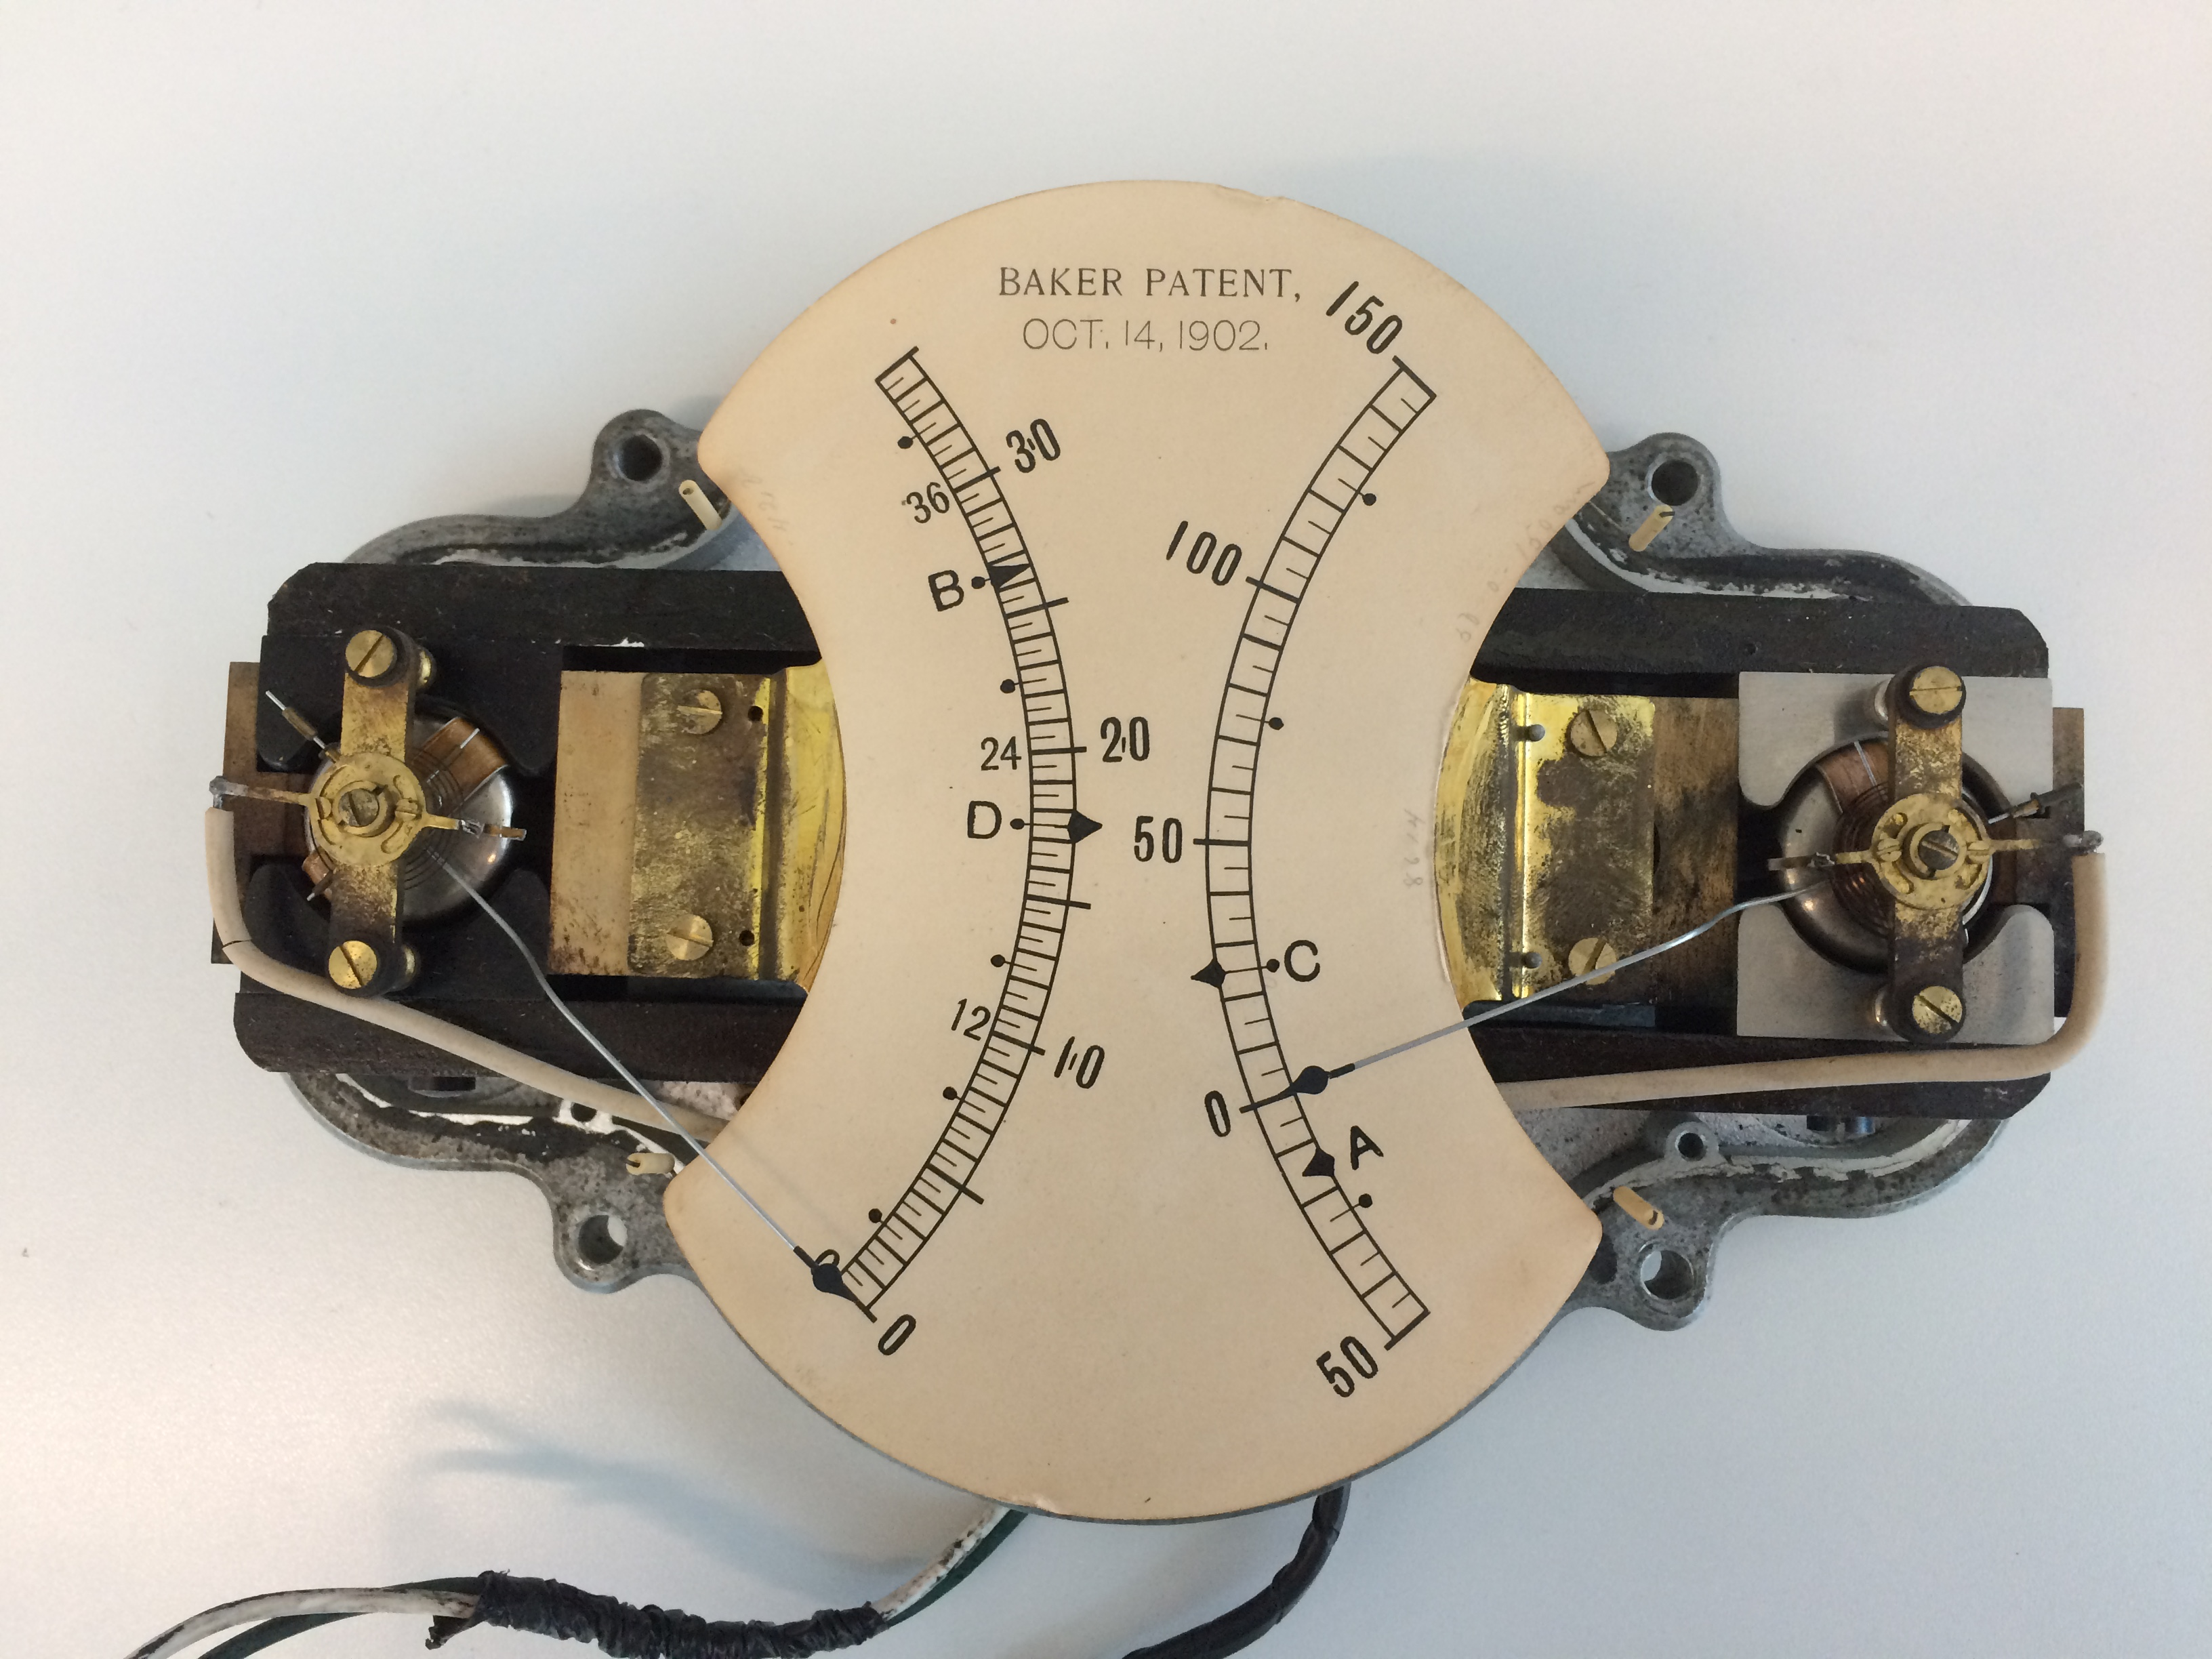
\includegraphics[width=1.30\textwidth]{images/Anhang/Volt_Ampere.jpg}
	\caption{\textcolor{blue}{Das ursprüngliche Anzeigegerät für Batteriespannung und -strom funktioniert auch im umgebauten Detroit}}
	\label{fig:Volt_Ampere}
\end{figure}
\begin{figure}[h]
	\centering
		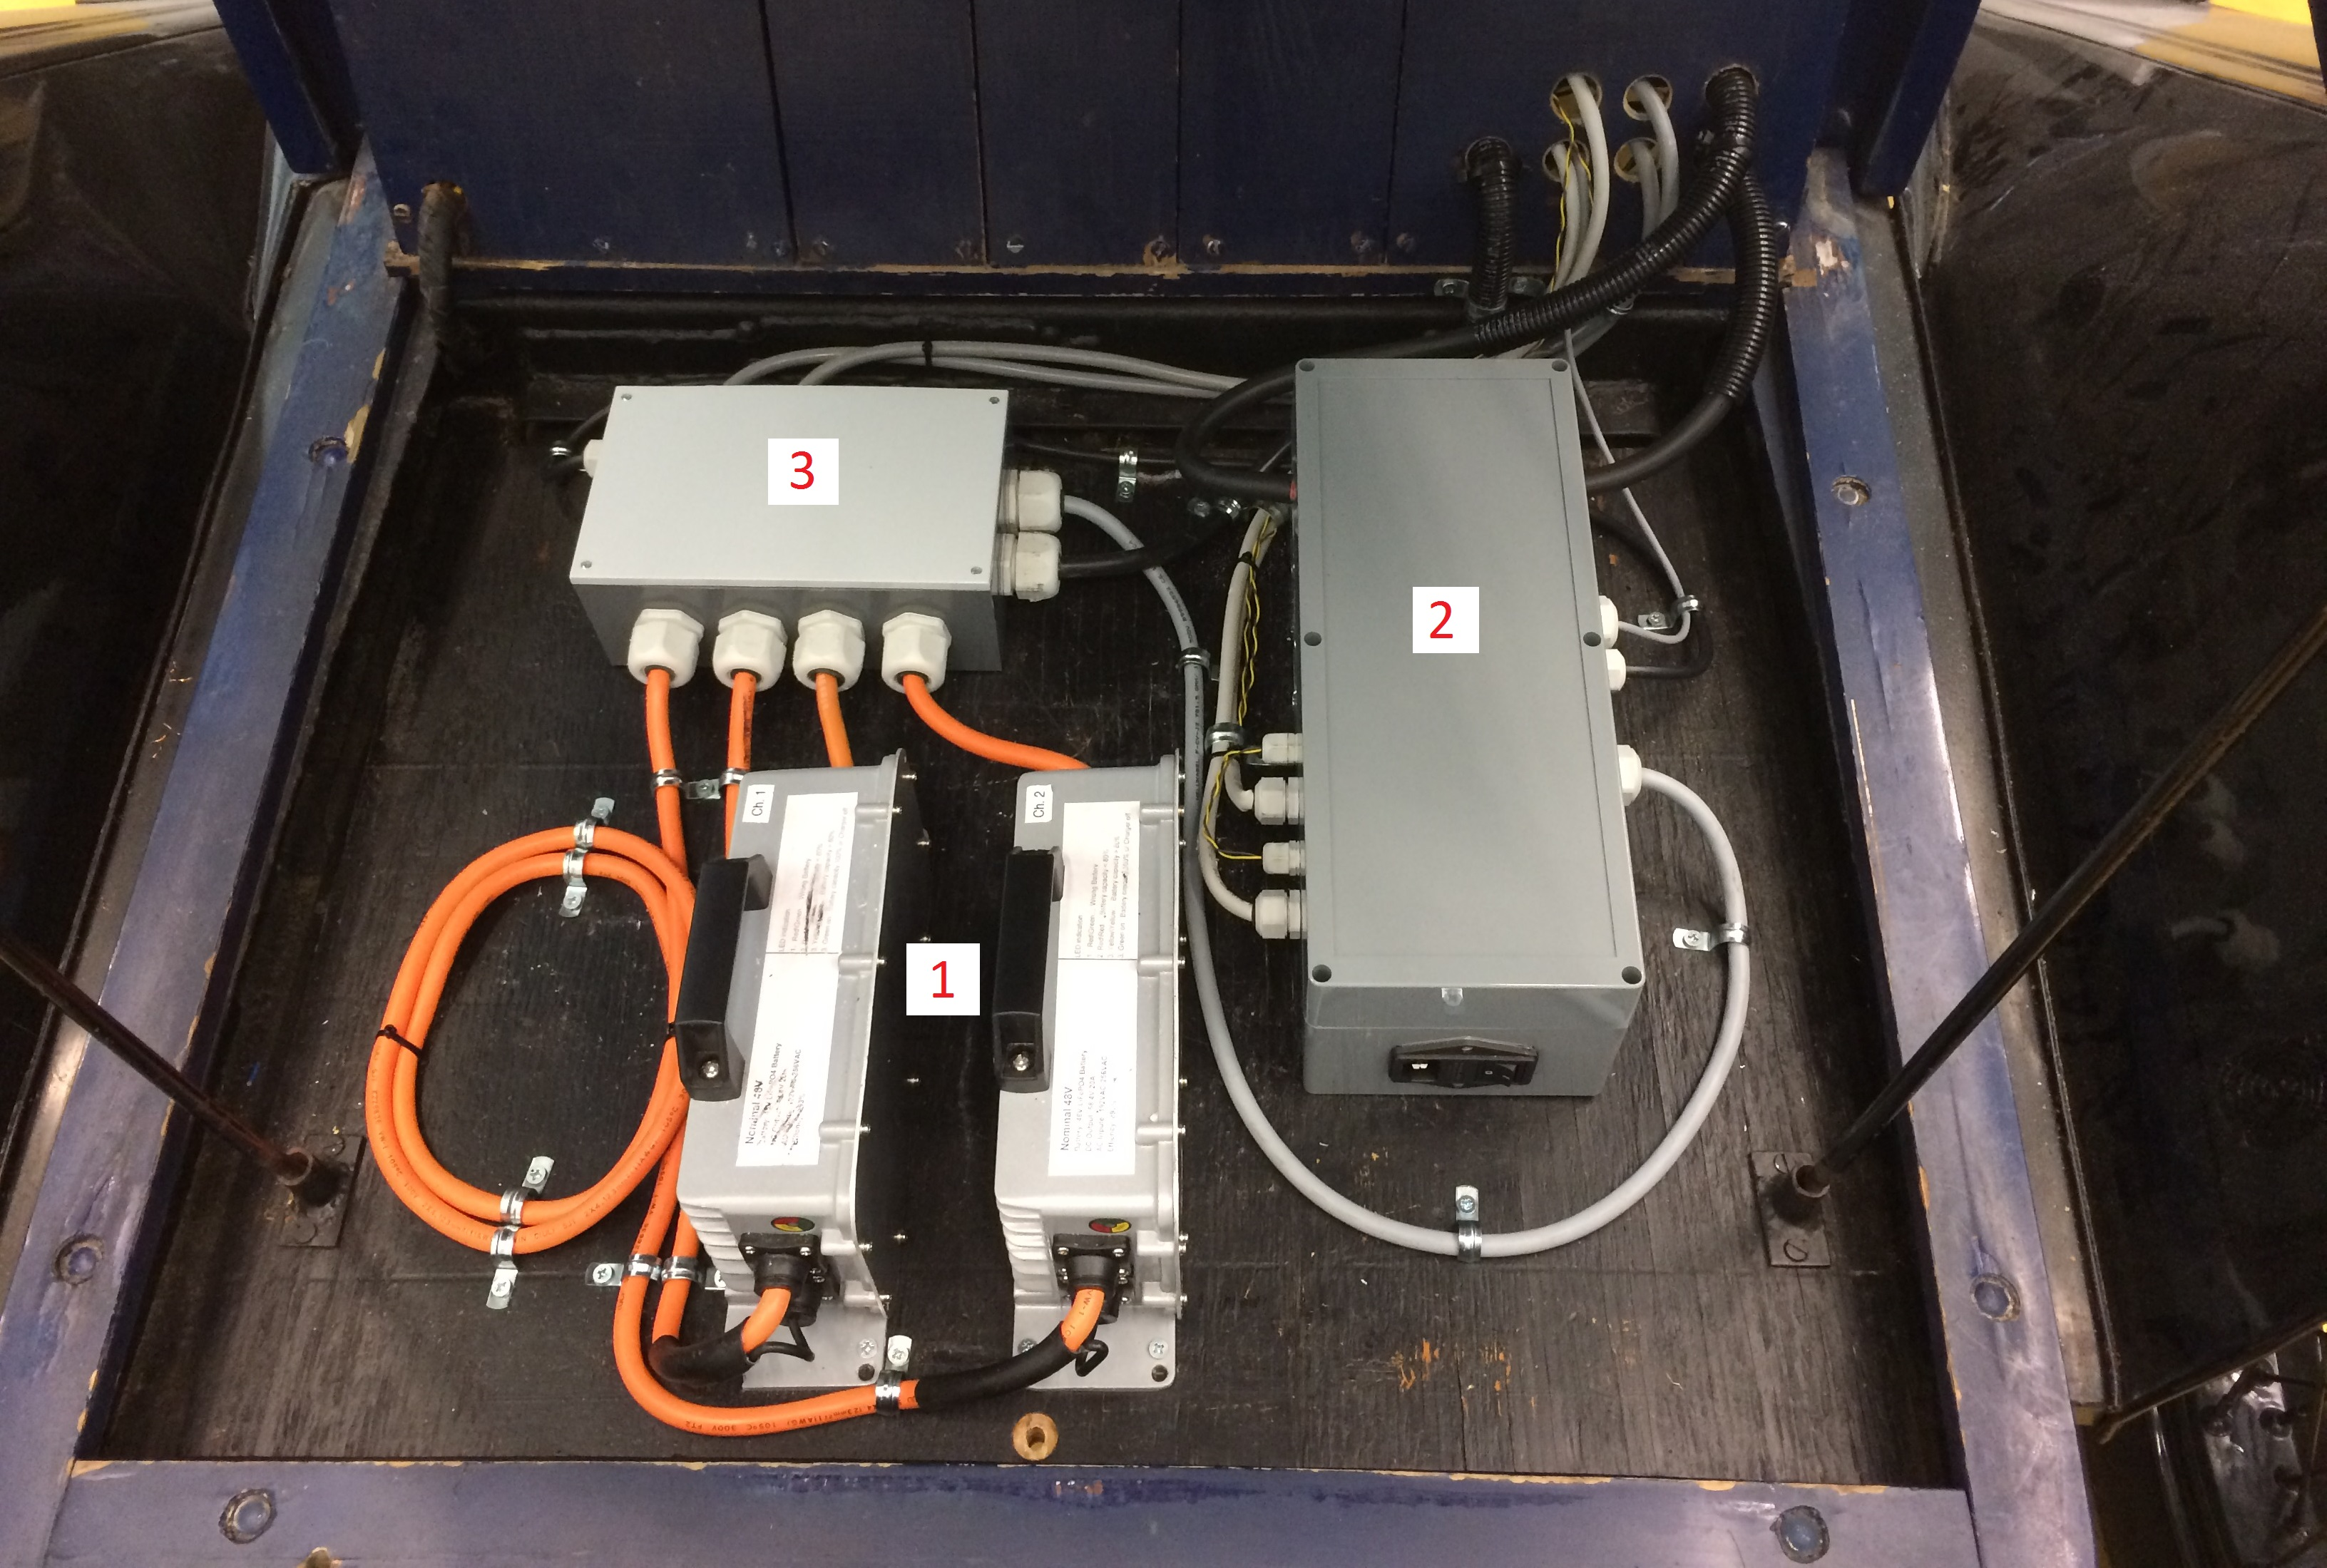
\includegraphics[width=1.30\textwidth]{images/Anhang/Front.jpg}
	\caption{\textcolor{blue}{In der Front ist die neue elektrische Ausrüstung, abgesehen von der Batterie, eingebaut: Die beiden Ladegeräte (1) laden beide Batterien unabhängig; die Steuerbox (2) kombiniert die Informationen der beiden Batterien und bereitet sie für das Fahrzeug auf, in ihr befindet sich ebenfalls der neue gasisolierte Hauptschalter; die Anschlussbox dient zum Verlängern der Leitungen der Ladegeräte zur Batterie, ausserdem wird von hier aus das Lichtsystem sowie der Not-Aus-Schalter eingespeist}}
	\label{fig:Front}
\end{figure}
\newpage
	\end{landscape}

